\chapter{Usage}

This chapter describes how to install X11-Basic on the most popular operating 
systems and how to run the interpreter and how to compile BASIC programs.

The X11-Basic interpreter is called \verb|xbasic| (\verb|xbasic.exe| under 
Windows). The compiler \verb|xbc| (\verb|xbc.exe| under  Windows). Under Unix
these executables are usually installed in the \verb|/usr/bin/| (if installed
via  the package management system) or in \verb|/usr/local/bin|  (if installed
manually from the source package) path. Under Windows, the files are installed
normally under the directory \verb|C:\x11basic|. Under Android you will not have
to care about the individual components of X11-Basic,  because there the
X11-Basic app comes with a little IDE  (Integrated Development Environment)
which handles the terminal, editor, loading running and the compile process 
for you.

\section{Installing X11-Basic}

For the most popular operating systems, ready-made packages are  available which
allow an easy installation of X11-Basic without the  need of compiling it from
source code. 

For other operating systems not mentioned here, X11-Basic may or may not work. 
Generally no binary package might be available, so in these cases you will have 
to compile all X11-Basic components (manually) by your own. You may be lucky 
and you are not the first trying this, so searching the internet for hints is 
generally a good idea.

But most likely you are reading this manual because you have already got 
X11-Basic installed on your system, or you at least have a package ready 
to be installed right away.

\subsection*{SuSE-Linux and RedHat}\index{RPM}

If you have got a Redhat-Package (RPM) e.g. a file named 
\verb|X11Basic-1.28-1.i386.rpm|, then you can install this package (being
root) with 
\begin{verbatim}
rpm -i X11Basic-1.28-1.i386.rpm      .
\end{verbatim}

This is a very convenient way at least for the Linux distributions  {\it
Feodora}, {\it Mandriva}, {\it SuSE} and {\it RedHat} (and maybe others,
basically derived distributions\footnote{A list of RPM based Linux distributions
can be found here:
\url{http://en.wikipedia.org/wiki/Category:RPM-based_Linux_distributions}}) to
install the interpreter, the compiler,  and its documentation, the man-pages and
a small collection of example programs. 

Following files will be normally installed:
{\footnotesize
\begin{verbatim}
/usr/bin/xbasic             -- the X11-Basic interpreter
/usr/bin/xbc                -- the compiler
/usr/bin/xbbc               -- bytecode compiler
/usr/bin/xvbm               -- bytecode interpreter (virtual machine)
/usr/bin/xb2c               -- the bytecode to C translator
/usr/bin/bas2x11basic       -- the ANSI BASIC to X11-Basic translator
/usr/lib/libx11basic.so     -- the runtime library (shared object)
/usr/lib/libx11basic.a      -- the runtime library for static linking
/usr/include/x11basic/x11basic.h -- the header file for library API
/usr/include/x11basic/xb2csol.h  -- the header file for compilation of xb2c output
/usr/share/man/man1/x11basic.1 -- the man-page of X11-Basic
/usr/share/man/man1/xbasic.1   -- the man-page of the X11-Basic interpreter
/usr/share/man/man1/xbc.1   -- the man-page of the compiler
/usr/share/man/man1/xbbc.1  -- the man-page of the bytecode compiler
/usr/share/man/man1/xbvm.1  -- the man-page of the virtual machine
/usr/share/man/man1/xb2c.1  -- the man-page of the X11-Basic to C translator
/usr/share/man/man1/bas2x11basic.1 -- the man-page of the ANSI to X11-Basic  translator
\end{verbatim}
}

After having installed the package, you can execute the interpreter 
with \verb|xbasic| or read the man pages with \verb|man xbasic| or 
\verb|man x11basic|.

The documentation should install into the 
\verb|/usr/share/doc/packages/X11Basic/| directory 
and you should find the following files:
{\footnotesize
\begin{verbatim}
-rw-r--r--    1005  ACKNOWLEGEMENTS      -- acknowledgments
-rw-r--r--      46  AUTHORS              -- contact addresses of the author
-rw-r--r--   17982  COPYING              -- copyright information
-rw-r--r--    2960  INSTALL              -- installation instructions
-rw-r--r--    1752  README               -- short description
-rw-r--r--     170  RELEASE_NOTES        -- release notes
-rw-r--r--  164370  X11-Basic-manual.txt -- the manual (txt version)
drwxr-xr-x    1024  editors/             -- files for editors / syntax highlighting
drwxr-xr-x    1024  examples/            -- few example programs
\end{verbatim}
}

\subsection*{Debian based distributions, Ubuntu and Knoppix}\index{Debian}

If your Linux distributions does not use the RedHat package system it is very
likely that it instead uses the Debian package system. The most popular Debian
based Linux distributions are {\it Knoppix} and {\it Ubuntu}\footnote{A list of
Debian based Linux distributions can be found here:
\url{http://en.wikipedia.org/wiki/Category:Debian-based_distributions}}. 

X11-Basic also comes in packages called (e.g.)
\verb|x11basic_1.28-64_i386.deb|. Usually you can very easily install the file
from a file browser with simply double clicking on it. Also a 
\begin{verbatim}
dpkg -i x11basic_1.28-64_i386.deb
\end{verbatim} 
from a terminal will do. The file system structure should be similar
to what is described in the previous chapter (explaining the RedHat packages),
so you should expect to find the same files at the same places. Please note, 
that you need a special Debian package if you want to install it on 64 bit Linux
installations, usually called \verb|x11basic_1.28-64_amd64.deb|. 

\subsection*{Other Linux and UNIX distributions}

The author currently provides only 32bit and 64bit Debian binary packages for 
Linux (specifically {\it Ubuntu Linux}). A
rpm package can be made out of the Debian packet with a tool called
\verb|alien|. 

For exotic Linux based devices usually binary distributions come as a zip file
(like the TomTom version). In these cases they are accompanied by a README or
other instructions how to install them. The package for Android comes in a file
called \verb|X11-Basic-1.28-64.apk| usually provided by F-Droid, the app store 
for free and open source software, which also installs it for you. 

For all other systems you will have to get the source-package 
\verb|X11Basic-1.28.tar.gz| and compile the sources. This should work for  all
Linux distributions, and probably with little modifications also for {\it
HP-UX} (Hewlett-Packard UniX), for DEC/alpha, for MAC/OSX, for SUN/SOLARIS and
FreeBSD and maybe others.  Also X11-Basic compiles on Cygwin, and on
ARM-Linuxes like the one often used together with the {\it Raspberry Pi}. 
Please note that X11-Basic is designed for 32-bit operating systems. 
X11-Basic will also compile on 64 bit systems. But some of the
functions may not work, especially pointer arithmetic (\verb|VARPTR()|, 
\verb|PEEK()|, \verb|POKE|, etc.)
will probably lead to segmentation faults when using huge amounts of 
memory.\footnote{In X11-Basic all pointers to memory addresses are stored in 
32bit integer variables. The upper 32bits of the addresses are stored internally
for further use. So if you calculate VARPTR(a), you would be able to 
POKE to the address immediately after without error, because the upper part of 
the addresses was stored internally from the previous call to VARPTR. 
X11-Basic will emit a warning, 
pointer base has changed, whenever this part is different from what it 
was before. This way, pointer arithmetics can be used with care, even on 64 bit 
operating systems.} It has turned out, that also the GEM AES graphics functions 
make use of pointer conversions (to stay compatible with the ancient ATARI ST format), 
also here a problem might occur. Also the statically linked versions of X11-Basic are
more likely to work correctly, because the shared libraries are loaded to the upper
address space. So If you see the WARNING messages, try to use a static version of 
X11-basic (\verb|xbasic.static|). 

\subsection*{Compiling X11-Basic from its sources under UNIX like systems}
\index{Compiling}

If you have a binary package of X11-Basic, you can safely skip this section.

In order to compile X11-Basic, you will need the following:

\begin{itemize}
 \item A C compiler, preferably GNU C (but other ANSI C compilers will do), 
 \item X11 libraries  (for the graphics) or a framebuffer device or the SDL library,
 \item optionally the \verb|readline| library, 
 \item optionally the \verb|LAPACK| library,
 \item optionally the \verb|GMP| library,  
 \item optionally the \verb|ALSA| sound library (\verb|libasound|) and/or the SDL framework.
\end{itemize}  

These will suffice to get you started. If one or more of these libraries are
not present on your system, the \verb|configure| and \verb|make| scripts will
try to compile a version, which does not need them (hence leaving out some of
the functionality of X11-Basic.).

\begin{enumerate}
\item Install the development environment packages, e.g. done by the command:
\begin{verbatim}
sudo apt-get install libx11-dev libreadline6-dev liblapack-dev \
             libgmp-dev libfftw-dev 
\end{verbatim}

\item Unpack \verb|X11Basic-1.28.tar.gz| with 
\begin{verbatim}
tar xzf X11Basic-1.28.tar.gz
\end{verbatim}
\item go into the \verb|X11Basic-1.28| directory and do a 
\begin{verbatim}
./configure
make
sudo make install
\end{verbatim}
\end{enumerate}
That's all you will have to do (for more detailed installation instructions read
the file INSTALL, which comes with the package.).

If the `configure' script fails, please contact me
(\url{kollo@users.sourceforge.net}) and send me the output it generated
(\verb|config.log|). I am going to try to help you to fix the problem.

\subsection*{Special comments on the framebuffer version}
\index{framebuffer}

Very useful on the Raspberry pi and other low memory/low resources computers 
is the option not to use X or SDL libraries at all. You can have a full 
featured X11-basic with graphics and mouse input anyway, if you compile the 
framebuffer version (\verb|make fb|). This will produce the single file 
\verb|xbasic.framebuffer| which is the interpreter (and virtual machine) 
ready to be used from a console (and without X). This way you have full control 
over the screen and mouse and keyboard. Usually everything you need to make the 
Raspberry pi interact with and display to the user. 

\subsection*{Cross-compiling other Versions of X11Basic}
\index{cross compiling}

The Makefile allows you to also produce the compiler (\verb|make xbc|),  the
bytecode compiler (\verb|make xbbc|), the virtual  machine (\verb|make xbvm|),
and the X11-Basic to C translator (\verb|make xb2c|). If you  need the separate
libraries you can do a \verb|make x11basic.a| and a \verb|make libx11basic.so|.
These libraries are for example needed by the compiler \verb|xbc|. 

If you want to make a version which uses the framebuffer (instead of the
X-Server) do a \verb|make fb|. If you want a version using the SDL library, do a
\verb|make sdl|.

The TomTom distribution can be generated with \verb|make TomTom|. (The ARM-Linux
cross-compiler is needed).

The MS WINDOWS distribution can be generated with \verb|make windows|. (The
mingw cross-compiler is needed).


\subsection*{Support}\index{Support}

If you have trouble with X11-Basic, you may send me a mail. Please understand
that I need to find time to answer your mails. On 
\url{http://sourceforge.net/projects/x11-basic/} there is a forum (bug reports,
patches, request for help, feature requests) about X11-Basic. You can as well
place your questions there, so that also other users of X11-Basic have a chance
to help. It is also worth browsing through the topics. Maybe someone has already
found a solution to your problem. It is as well ment for the users to
share their experience with other X11-Basic users.

If you have trouble with some X11-Basic command or program, and you think it is
a bug in the X11-Basic interpreter or compiler itself, you should create  a
minimum sample program to reproduce the error; please keep this sample  program
as small as possible. Then take the program and send it to me. Add a short
description of you problem, containing:  
\begin{itemize} 
  \item Which operating system are you using: Windows or UNIX, Linux, Android?  
  \item How does the program behave on your computer? What did you expect?  
  \item Which version of X11-Basic are you using? Please try the latest one! 
\end{itemize}

\section{Using the X11-Basic Interpreter}

There are several ways to start the X11-Basic interpreter depending on the
operating system you are using it.

\subsection{Using the X11-Basic Interpreter under UNIX, Linux}\index{UNIX}\index{Linux}

The simplest way is to just start it by the command \verb|xbasic| from a
terminal window or a console. Then you can use the interpreter in interactive
mode. Just try to enter some X11-Basic commands. The interpreter itself also
accepts several options via the command line. Please also read the man-page
(\verb|man xbasic|) for more details.

In Ubuntu or Lubuntu you will also find X11-Basic in the start menu. When you
select  X11-Basic from the start menu, the interpreter should come up in its own
terminal window. 

\subsubsection{X11-Basic as a shell}\index{shell}

X11-Basic programs can be executed like shell scripts. Make sure that the very
first line of your X11-Basic program  starts with the characters \verb|'#!'|
followed by the full pathname of the X11-Basic interpreter \verb|xbasic| (e.g.
\verb|'#!/usr/bin/xbasic'|).  This she-bang line ensures, that your UNIX will
invoke \verb|xbasic| to  execute your program. Moreover, you will need to change the
permissions of your X11-Basic program, e.g. \verb|chmod 755 myprog.bas|.  After
that your program can simply be executed from your shell and the interpreter
works in the background like shells do. You need not even use the extension .bas
for your scripts.

\begin{mdframed}[hidealllines=true,backgroundcolor=blue!20]
\subsubsection*{Example: draftit} A tool to stamp a postscript file
with "draft" on every page.
{\footnotesize
\begin{verbatim}
#!/usr/bin/xbasic
i=1
WHILE LEN(PARAM$(i))
  inputfile$=PARAM$(i)
  INC i
WEND
CLR flag,count
IF NOT EXIST(inputfile$)
  QUIT
ENDIF  
OPEN "I",#1,inputfile$
WHILE NOT EOF(#1)
  LINEINPUT #1,t$
  IF count=3
    PRINT "%% Created by draftit X11-Basic (c) Markus Hoffmann from "+inputfile$
  ENDIF
  IF GLOB(t$,"%%Page: *") AND NOT GLOB(t$,"%%Page: 1 1*")
    IF flag
      PRINT "grestore"
    ENDIF
    flag=1
    PRINT t$
    PRINT "gsave"
    PRINT ".80 setgray"
    PRINT "/Helvetica-Bold findfont 140 scalefont setfont"
    PRINT "0 80 800 { 306 exch moveto"
    PRINT "(Draft) dup"
    PRINT "stringwidth pop 4 div neg 0 rmoveto 6 rotate show } for"
    PRINT "grestore"
  ELSE 
    PRINT t$
  ENDIF
  INC count
WEND
CLOSE
QUIT
\end{verbatim}
}
\end{mdframed}

\subsection{Using the WINDOWS Version of X11-Basic}

The installation is done in the usual way with a setup program, e.g.
\verb|X11-Basic-1.28-64-setup.exe|, which you can download from the homepage.
All files will be installed on the program folder on `C:`.

In the case you have got a .zip file, e.g. \verb|X11-Basic-1.28-64-win.zip|, 
you should extract all files and invoking the setup program (\verb|setup.exe|). 
This installs X11-Basic into a folder  \verb|C:\\x11basic|.  
All files you need for
using X11-Basic are located there:

\begin{verbatim}
  lib           -- empty folder for future use
  bas.ico       -- the icon for .bas files
  demo.bas      -- one of the example programs
  readme.txt    -- short description of X11-Basic
  SDL.dll       -- the Simple Direct Media Library
  setup.exe     -- Installation and uninstall program
  x11basic.ico  -- another X11-Basic icon
  X11-Basic.pdf -- The X11-Basic User Manual
  xb2c.exe      -- bytecode to C translator
  xbasic.exe    -- The X11-Basic interpreter
  xbc.exe       -- The X11-Basic compiler
  xbvm.exe      -- The virtual machine
\end{verbatim}

X11-Basic can be invoked in the following three ways:

\begin{enumerate}
\item Choose "X11-Basic" from the start-menu: You can choose between 
\begin{description}
\item[COMPILER]: opens the compiler Application which then asks for a .bas file to compile into .exe,
\item[DEMO]: Opens and runs the demo.bas example program,
\item[DOCU]: Opens the X11-Basic User Manual,
\item[X11-Basic]: Opens the X11-Basic interpreter. \verb|xbasic.exe| will come 
up with a console window and the interpreter waits for commands to be typed
in right away.
\end{description}
\item Click with the right mouse button on your desktop. Choose "new" from the 
      context menu that appears; this will create a new icon on your desktop. 
      The context menu of this icon has three entries "Execute", "Edit" and   
      "View docu" (which shows the embedded documentation, if any); a         
      double-click executes the program.
\item Create a file containing your X11-Basic program. This file should have    
      the extension ".bas". Double-click on this file then invokes X11-Basic,   
      to execute your program. 
\end{enumerate}

The compiler has a rudimentary graphical user interface, which will ask for 
the .bas file to be compiled and later for the name of the executable to be 
written to.

By default, the WINDOWS or DOS console does not support ANSI/VT100 coding.  So
\verb|PRINT AT()| and line editing will probably not work. To fix this,
ANSI.SYS  has to be installed and switched on for the console windows.
Instructions how to install \verb|ANSI.SYS| can be found on the Internet. 
(Also an alternative extension named ANSICON can be used.)

\subsubsection*{The Context Menu}\index{context menu}

Every icon under WINDOWS offers a context menu when you click on it with the
right mouse button. Clicking on an icon of a X11-Basic program as well opens this 
context menu with following options: 
\begin{description}
\item[Execute] will invoke the X11-Basic interpreter to execute your program. 
The same happens, if you double-click on the icon.
\item[Edit] invokes {\it notepad}, allowing you to edit your program.
\item[View docu] opens a window which shows the embedded documentation 
of your program if there is any. Embedded documentation within a .bas file are comments, which
start with a double comment character (\verb|##|).
\end{description}

\subsection{The Android Version of X11-Basic}\index{Android}

A version of X11-Basic ready to be installed on Android smart-phones and tablets
is available on the {\it F-Droid app store}. 
A more recent version usually can be found in the releases section of the project 
pages of X11-Basic on codeberg. Watch out for a file named 
\verb|X11-Basic-1.28-64.apk| which contains the app.  Download this file to 
your Android tablet or smart-phone and install it, allowing installation 
of apps from other sources in the systems settings before if necessary.

Unlike the other versions of X11-Basic, the interpreter and virtual machine is
embedded in a little IDE (=Integrated Development Environment) which allows the
user to load, run, edit and compile the programs.\index{IDE}

The app registers itself as a viewer to .bas and .b files on the system. So
from any file browser, basic programs can be started with a single touch. 

If you open the X11-Basic app itself, you can directly type in commands with
the virtual keyboard. Pressing the MENU button gives you the option to load and
run BASIC programs, stop and continue execution, open the keyboard (if its has
vanished from the screen) and compile basic programs into bytecode. The virtual
machine is integrated, so bytecode compiled code can be run. Depending on the
endianess of the processor architecture of the platform, bytecode may or may not
be compatible with those produced on a Linux PC or WINDOWS machine. Standard
output is rendered directly into the graphics screen with a VT100\index{VT100} compatible
terminal emulation. Not all graphics features have the same result than on a
X11-Windows installation, the whole screen counts as a single full-screen
window. Finally shortcuts to X11-Basic programs can be placed on the desktop,
so they can be started with one click. Also X11-Basic is registered as a method
to open files (from a file browser).  A small selection of example programs is
included in the Android package. If you like to have some fun with a game, try
\verb|ballerburg.bas|.

\subsubsection{Usage on Android devices}

Android devices usually have a BACK button, a HOME button and a MENU button. 
\begin{itemize}
\item The HOME button suspends X11-Basic and returns to the Android desktop. 
      Selecting the X11-Basic app again will resume it. If a BASIC 
      program was running, it will continue to run in the background.
\item With the BACK button, a running BASIC program will be stopped. 
      If you press the BACK button again, the X11-Basic interpreter quits.
\item The MENU button opens a menu with following options: About, LOAD program,
      RUN program, STOP/CONT program, NEW, Keyboard, Paste from clipboard, 
      Info/Settings, Editor, Compile and Quit.
\begin{description}
\item[About] shows information about the current version of X11-Basic, news and 
             impressum.
\item[Load ...] opens a file-selector which displays all .bas and all .b 
                programs in the directory \verb|/mnt/sdcard/bas|. 
		The selected program will be loaded into memory. A program 
		eventually stored there before will be overwritten. You can 
		display the source-code by entering \verb|LIST|.
\item[Run] will simply start the execution of a program which has been 
             loaded before. (You can also enter RUN)
\item[STOP/CONT] will interrupt the execution of the program or resume it. 
                 (you can also press the BACK button once to stop the program, 
		 and you can enter \verb|CONT| to continue it).
\item[New]      will delete the currently loaded program from memory.
\item[Keyboard] will show or hide the on-screen virtual keyboard. If you have 
                a hardware or external USB/Bluetooth keyboard, you can also 
		enter commands with that.
\item[Paste from Clipboard] will paste any text you have copied to the 
                            clipboard (from any other application) before.
\item[Info/Settings] will open a dialog with additional information, links, 
and preference settings. The preferences can be set as follows:
\begin{description}
\item[Show splash screen at X11-Basic start-up.] This can be switched off here.
\item[Select screen focus.] When the screen will be partially covered by the 
    on-screen virtual keyboard, you can specify which portion of the screen 
    should be visible: The top portion, bottom portion, the whole screen but 
    scaled to fit, the portion with the text cursor in it, or the portion with 
    the mouse pointer in it. The default is: scaled.
\item[Select font size.] If the screen is small, but the resolution is high, 
you may want to change the font size to LARGE. This setting affects the 
console font (text mode) as well as the graphics/user-interface appearance.
\end{description}
\item[Show title] This can be switched off here.
\item[Show status bar] This can be switched off here.
\item[Show keyboard at start] This can be switched off here.
\item[Editor] will execute a 3rd-party text editor (e.g. {\it Ted} or 
{\it Jota} or {\it 920 Text Editor} if installed) to edit the program currently 
loaded. If no program 
was loaded, the default file name will be \verb|new.bas|. After having saved 
and closed the text editor, the modified program will be automatically 
reloaded into the X11-Basic interpreter.
\item[Compile] will compile the basic source code into bytecode which can be 
executed about 20 times faster (but cannot be edited or merged anymore). 
The bytecode will be saved with .b extension in the bas/ folder.
\item[Help] will open a window in which you can search the command reference.
\item[Quit] will terminate the X11-Basic interpreter.
\end{description}
\end{itemize}

\subsubsection*{Editing a program}
If you want to edit an existing program, do following steps (in this example, the editor used is TED, but it works similar with
Jota or many other text editors.):
\begin{enumerate}
\item Load an existing program with Menu --> Load,
\item choose Menu $\rightarrow$ Editor to edit the program, 
\item finish editing (and save it in the editor). Leave the editor by choosing EXIT in the menu or by using the BACK button (do not use the HOME button).
\item The program gets automatically reloaded, 
\item choose menu $\rightarrow$ run to run it.
\end{enumerate}

If you want to create a new program, follow these steps  (in this example, the editor used is TED):

\begin{enumerate}
\item Do a MENU -> New
\item Do a MENU -> Editor. The editor will be executed with the default file name (new.bas). 
If you have more than one editors installed, you will be asked which one to use. Select TED Text Editor.
\item Inside the editor do a "Save As" and give it a different name, e.g. "mything.bas", make sure that it is saved 
into the folder "bas".
\item Press the back button (not the HOME button), so the editor returns to X11-Basic.
\item X11-Basic now reloads new.bas, but this is not what you want, so
\item within X11-Basic load "mything.bas"
\end{enumerate}
The next time you edit it, it has the correct name, and a regular save in the editor should do
 as well as automatic reload in X11-Basic.

If you get an error when calling the text editor, you need to install one. There
are plenty around, e.g. {\em 920 Text Editor} or {\em Ted (tiny text editor)}.
Install them from the Android market. You can install multiple editors. Then you
are asked which one you like to use every time you call the editor.

\subsubsection*{LOAD file select functions}\index{LOAD}

To load a program, press menu --> load. You can now select a program file 
(either .bas or .b) to load. If you touch the filename long you get another 
menu with advanced functions: 
\begin{description}
\item[LOAD] -- load the program.
\item[MERGE] -- merge the program to the one already loaded (works only with .bas files).
\item[LOAD + RUN] -- load the program and immediately run it.
\item[LOAD + LIST] -- load the program an list it.
\item[LOAD + edit] -- load the program and immediately start the editor.
\item[LOAD + compile] -- load the program and compile it.
\item[compile + RUN] -- compile the program and immediately run the compiled program.
\item[delete]   -- delete the selected file (you will be asked to confirm).
\item[CANCEL]   -- return to the file menu.
\end{description}

These functions are here for convenience only. You probably want to use LOAD+RUN
or compile+RUN more often.

\subsubsection*{Running in the Background}

When a program is running and you press the home button, the program
will continue to run in the background. If you select X11-Basic app
again, it brings up the screen output.

Also: When you rotate the screen the running program should continue to run. It
needs to find out by using \verb|GET_GEOMETRY| if the screen size has changed. 

\subsubsection*{Desktop shortcuts}\index{desktop shortcuts}

You can create desktop shortcuts to your BASIC programs. You can place an
application shortcut on the home screen by simply pressing anywhere (and hold
for 1 second) on the background of the desktop screen (on Android 4.x devices go
to Apps $\rightarrow$ Widgets).  You first are asked to place the shortcut somewhere on the
desktop. The X11-Basic launcher then asks for a .bas or .b file and places the
link on the desktop. Pressing this link will automatically load X11-Basic and
the .bas program and run it.

You can select any file from the \verb|/sdcard/bas| folder which then is placed in the
desktop.

\subsubsection*{Updates of example programs}\index{example programs}

The X11-Basic app comes with a small selection of example programs. They are 
copied into the \verb|/mnt/sdcard/bas/| directory. The X11-Basic app will never
overwrite a file in \verb|bas/| which is already there. If you want a specific
example program be updated (replaced with a potentially newer version, which has
come with an update of the X11-Basic app), simply delete the file. It will be
restored after the next execution of X11-Basic.


\subsubsection*{Troubleshooting the Android Version}
\begin{description}

\item[SCREEN REFRESH PROBLEM:] (Was reported sometimes on Samsung Tabs, 
all Android versions) e.g. galaxy note 1, Android 4.1.2:
{\bf Symptoms:} Running the X11-Basic app, the screen output is not updating or 
refreshing while X11-Basic runs a program. 
{\bf CURE:} you should check the system settings:
\begin{verbatim}
Developer settings -->  deactivate Hardware overlays: ON 
                   -->  force Gpu: OFF 
\end{verbatim}

\item[Characters typed are not visible] If the whole line appears  after you
pressed ENTER, but you like to see what you are typing, you  need to modify the
settings of the keyboard (switch off auto-completion  and anything like that,
which may make the keyboard hold text back until you press enter.) If still 
nothing appears after ENTER, then you probably have the Screen Refresh Problem 
(see above).

\end{description}

%\subsection{The TomTom Version of X11-Basic}
%
%On \url{http://www.opentom.org/X11-Basic} you will find a version of X11-Basic
%which has been specially compiled for TomTom navigation devices. They run Linux
%based on the ARM processor. A ready made package as well as installation
%instructions can be found on that web-site. Currently only versions  1.14, 1.15
%and 1.18 of X11-basic are available as a ready-made binary package. Since the
%new versions of TomTom devices do not allow to install any third party apps
%anymore, the support for TomTom has been given up (in 2011).

\subsection{Command line parameters}\index{command line parameters}

If you are using X11-Basic under Android, you can skip this section. 
Command-line parameters cannot be used on Android.

The X11-Basic interpreter \verb|xbasic| can be evoked with  additional but
optional command line parameters. It takes the following ones:

\begin{longtable}{lp{11cm}}
  {\tt\bf xbasic} {\it<filename>} & run Basic program \verb|[input.bas]|\\
  \verb|-l|                       & load only, don't execute\\
  \verb|-e| {\it<command>}        & execute basic command \\
  \verb|--eval| {\it<expression>} & evaluate numerical expression  \\
  \verb|--daemon|                 & switch off prompting and echoing\\
  \verb|-h --help|                & print a short help \\
  \verb|--help|  {\it<topic>}	  & print help on a specific topic\\
  \verb|--quitonend|              & changes the behavior of the interpreter such 
  that it quits after the program  has  finished.
  The direct mode / interactive mode will not be entered.\\
\end{longtable}

\begin{mdframed}[hidealllines=true,backgroundcolor=black!20]
\subsubsection*{Examples:}
\begin{verbatim}
  xbasic testme.bas
  xbasic -l dontrunme.bas
  xbasic -e 'ALERT 1,"Hello !",1," OK ",b'
  xbasic --eval 1+3-4*3
\end{verbatim}
\end{mdframed}

\subsubsection*{X11-Basic as daemon}

The command line option {\bf \verb|--daemon|} forces the interpreter to run in
daemon-mode (with no terminal connected). No prompt is given and the 
input is not echoed back. This is useful, if you want to run X11-Basic
programs as a background service.
  
%\subsection*{Example:}
%To run  the X11-Basic interpreter on a tcp-socket on port 1371 create a new 
%user called {\normalfont \bf xbasic} and insert
%{\footnotesize
% \begin{verbatim}
%       --- in /etc/inetd.conf: ---
%       xbasic stream tcp nowait xbasic /usr/sbin/tcpd /bin/xbasic --daemon
%       --- in /etc/services: ---
%       xbasic          1371/tcp
%       ---
%  \end{verbatim}
%}
%
%Please note that this example is just for demonstrations. X11-Basic should not
%really be used in that way, because \verb|xbasic| would open several security
%holes on your system.

\subsubsection*{Additional command line parameters for the framebuffer version}

If X11-Basic was compiled to use the framebuffer device for graphics output there are
three more options to control which framebuffer device is to be used, which mouse 
device and which keyboard-device:

\begin{longtable}{lp{11cm}}
\verb|--keyboard| {\it<device>} & set the keyboard device (default: \verb|/dev/input/event4|)\\
\verb|--mouse|    {\it<device>} & set the mouse device (default: \verb|/dev/input/mice|)\\
\verb|--framebuffer| {\it<device>} & set the framebuffer device (default: \verb|/dev/fb0|)\\
\end{longtable}

For example: The sense hat for the Raspberry Pi uses the framebuffer device
\verb|/dev/fb1| for its LED matrix. So if you want to draw to the LED matrix 
display specify this for graphics output.
\begin{mdframed}[hidealllines=true,backgroundcolor=black!20]
\begin{verbatim}
  xbasic --framebuffer /dev/fb1 led-blink.bas
\end{verbatim}
\end{mdframed}


\section{Editing X11-Basic programs}\index{Editor}

X11-Basic programs (source code, \verb|.bas| files) are regular ASCII files and
therefore can be created with any text editor available.  

%MS-WINDOWS users
%should make sure, that the line ending character is set to Unix style  (only
%\verb|CHR$(10)|) and not WINDOWS (or ATARI ST) style  \verb|CHR$(13)+CHR$(10)|).
%Therefore the WINDOWS built-in notepad application  should not be used. Use {\it
%notpad2} instead. 
Users of UNIX like operating systems are fine with every text editor. Simple 
ones like \verb|pico| or \verb|nano| will do. MS-WINDOWS user can use the simple 
{\it notepad} text editor.

Users of X11-Basic under Android need to install a good text editor. TED (Text
Editor), \verb|920 Text Editor|, or \verb|Jota| will work fine. Other text
editors which might have been already preinstalled can be a source of
frustration and trouble. So if unsure, please install one of the mentioned
editors. If you have installed more than one editor,
this is no problem, you will be asked which one to use every time the editor
is invoked. 

Besides from the basic editing features I recommend to use a text editor with
syntax highlighting. Currently X11-Basic syntax definitions are available for 
\verb|nano| (available for the text consoles) and for the {\it
Nirvana Editor} (\verb|nedit|, available for Linux, UNIX and WINDOWS)  as well
as for the \verb|920 Text Editor| and \verb|Jota|, available for Android.

X11-Basic can support foreign language characters. Therefor the basic program
may be coded in UTF-8 which is compatible to ASCII but has the ability to use
and encode any Unicode character. Such characters can be used in X11-Basic
string constants, but may not be used in variable names. Currently only the
standard output (console) supports the full UTF-8 character
sets.\footnote{LTEXT will accept some of the special characters
(currently only german), TEXT will work with UTF-8 only on Android
devices (all latin, greek, cyrillic).}

\subsection*{Using syntax highlighting with {\bf nedit}}\index{syntax highlighting}

NEdit, the full featured, plain text {\it Nirvana 
editor}\footnote{\url{http://nedit.org/}} is a GUI style text editor for
workstations with the X Window System.  Also a MS Windows port is
available\footnote{ \url{http://nedit.gmxhome.de/winport.html}}. NEdit provides
all of the standard menu, dialog, editing, mouse support, macro extension
language, syntax highlighting, and a lot other nice features (and extensions for
programmers). In short, it has everything you want to develop your X11-Basic
programs. Unfortunately nedit does not support UTF-8.

\begin{SCfigure}
\includegraphics[width=0.5\textwidth]{nedit-x11basic.eps}
\caption{The Nirvana Editor with syntax highlighting for a X11-Basic program.}
\label{nedit}
\end{SCfigure}

If you like to use \verb|nedit| as your favorite editor, a \verb|nedit.defs| file
comes  with this package. This enables syntax highlighting for X11-Basic
programs in {\bf nedit} (see fig.~\ref{nedit}).

\subsection*{Using syntax highlighting with {\bf nano} and {\bf pico}}\index{syntax highlighting}

GNU \verb|nano| is a text editor for Unix-like computing systems or operating 
environments using a command line interface. It emulates the \verb|pico| text
editor, part of the \verb|pine| email client, and also provides additional
functionality. Al though nano has to be used on the console, it can also use
pointer devices, such as a mouse, to activate functions that are on the shortcut
bar, as well as position the cursor. And most important, it can handle UTF-8.

\begin{SCfigure}
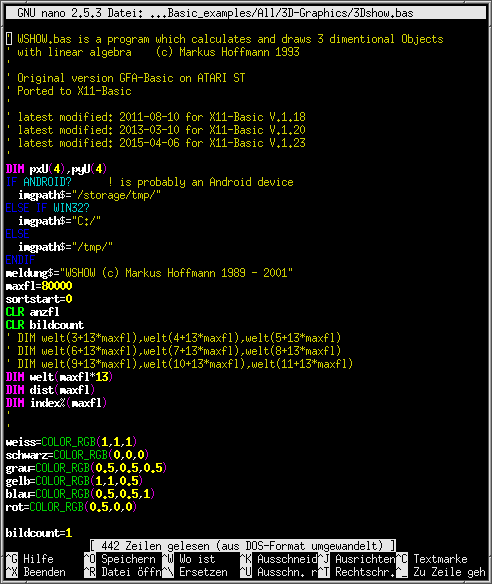
\includegraphics[width=0.5\textwidth]{nano-x11basic.eps}
\caption{The {\bf nano} editor with syntax highlighting for a X11-Basic program.}
\label{nano}
\end{SCfigure}

If you like to use \verb|nano| as your favorite editor, a 
\verb|x11basic.nanorc| file comes with the X11-Basic package. This enables
syntax highlighting for  X11-Basic programs in {\bf nano} (see fig.~\ref{nano}).



\section{The Byte-code Compiler and the Virtual Machine}\index{bytecode}

If you are using the Android version of X11-Basic, you can skip this chapter.
All you need to know is that there is the option to compile X11-Basic programs
(to byte-code) which makes them run much faster.

Under UNIX, Linux and Windows a separate program need to be used to compile .bas files and make byte-code files or 
standalone .exe files out of it. 

If you are using WINDOWS, the most convenient way to compile X11-Basic programs
is to execute the compiler \verb|xbc.exe| which has a little use interface. Also
under UNIX/Linux it is very convenient to use the compiler manager \verb|xbc|
with appropriate command line options (watch out for the 
\verb|-virtualm| option). 

Advanced users probably want to deal with the byte-code files produced in the
compiling process. For each compilation step there are separate programs which
do it; namely: \verb|xbbc|, \verb|xb2c| and \verb|xbvm|.

\verb|xbbc| compiles X11-Basic programs (.bas files) to byte-code files (.b).\index{xbbc}
\verb|xb2c| can translate byte-code files to C source code.\index{xb2c}
\verb|xbvm| is a virtual machine (interpreter for byte-code).\index{xbvm}

The idea is to increase the execution speed of X11-Basic programs a lot by 
compiling it to a byte-code, this still being portable. The byte-code itself is 
interpreted by a byte-code interpreter (also called a virtual machine). This
virtual machine needs to be present on the target computer, and then all
byte-code programs can be used there. This way, the X11-Basic compiler need not
deal with different target machine architectures, and also the byte-code can be
run much faster than the interpreted BASIC source code. 

The conversion to byte-code is a real compilation. The step to assembler or
machine code is not far. Also a translation to C or to JAVA or any other
language will be straight forward. As with JAVA, the byte-code is platform
independent and can be run on any system, which has a virtual machine ported to.

Also one point to mention (whether this is a feature or a disadvantage): 
X11-Basic byte-code can not be converted back into BASIC source code (.bas), but
is rather a very abstract representation of your program.

If you want to get a feeling on what this is about, open a .c source file, 
which has been produced by the byte-code to C translator \verb|xb2c|. Implemented
with an  additional macro translation step, the byte-code is in a way readable.
Here is an example:

\index{bytecode}
\begin{mdframed}[hidealllines=true,backgroundcolor=green!20]
{\footnotesize
\begin{verbatim}
...
    PUSH2;              /* 2  */
    ZUWEIS(2);          /* I= */
LBL_38:  PUSHV(2);      /* I */
    X2I;
    PUSHARRAYELEM(3,1); /* F(.) */
    X2I;
    JUMPIFZERO LBL_91;	/* JEQ(0x91); */
    PUSH2;              /* 2 */
    PUSHV(2);           /* I */
    EXCH;
    X2F;
    MULf;
    PUSHV(0);           /* S */
    LESS;
    JUMPIFZERO LBL_81;	/* JEQ(0x81); */
    PUSH2;
    PUSHV(2);           /* I */
    EXCH;
    X2F;
    MULf;
    ZUWEIS(5);          /* K */
LBL_61:  PUSHV(5);      /* K */
    X2I;
    PUSHVVI(3,1);       /* F */
    PUSHCOMM(30,1);     /* CLR */
    PUSHV(5);           /* K */
    PUSHV(2);           /* I */
    ADD;
    DUP;
    ZUWEIS(5);          /* K */
    PUSHV(0);           /* S */
    GREATER;
    JUMPIFZERO LBL_61;	/* BEQ_s(-29); */
    PUSHCOMM(74,0);     /* FLUSH */
LBL_81:  PUSHX("I"); 
    PUSHLEER;
    PUSHCOMM(147,2);    /* PRINT */
    PUSHVV(4);          /* C */
    COMM_INC;           /* INC */
LBL_91:  PUSHV(2);      /* I */
    PUSH1;
    ADD;
    DUP;
    ZUWEIS(2);          /* I= */
    PUSHV(0);           /* S */
    GREATER;
    JUMPIFZERO LBL_38;  /* BEQ_s(-104); */
...
\end{verbatim}
}
\end{mdframed}
This is bytecode made out of the (X11-Basic) lines:
\begin{mdframed}[hidealllines=true,backgroundcolor=blue!20]
{\footnotesize
\begin{verbatim}
...
FOR i=2 TO s
  IF f(i)
    IF 2*i<s
      FOR k=2*i TO s STEP i
        CLR f(k)
      NEXT k
      FLUSH
    ENDIF
    PRINT i,
    INC c
  ENDIF
NEXT i
...
\end{verbatim}
}
\end{mdframed}

You are not supposed to understand any of these, but it may give you a 
feeling about what byte-code really is, and that is really hard to reconstruct
the original BASIC lines out of it.

Please try the byte-code compiler out and maybe you want to report errors etc.
Quite a lot of the example programs are known to work well with the byte-code
compiler:  e.g. \verb|mandel-simple.bas|. The byte-code will execute about 10
times faster than the interpreted program. Here is how to use it:

\begin{mdframed}[hidealllines=true,backgroundcolor=black!20]
\begin{verbatim}
xbbc myprogram.bas -o b.b
xbvm b.b
\end{verbatim}
\end{mdframed}

\section{Using the X11-Basic to C translator}\index{C}

It is possible to translate the byte-code generated by \verb|xbbc|\index{xbbc} to C source
code and finally compile this intermediate C-source to a native executable
(e.g. with the GNU C compiler \verb|gcc|). This way the program will be a real
native executable which  --again-- runs even a bit faster  that the byte-code
interpreted by the virtual machine. 

Such programs can be linked against the dynamic library (.so or .dll) or the
static library (.a or .lib). In the end they run independently of any
interpreter or virtual machine.   However, some restrictions to the code apply.
Which means: not every program, which can be interpreted, can also be compiled.

The generated C-sources depend on the header file \verb|xb2csol.h| (normally 
installed under \verb|/usr/include/x11basic/|) the \verb|x11basic.a|  or 
\verb|libx11basic.so| libraries, which therefore should be present.  

\verb|xb2c| processes one input file. The suffix of the input file is  usually
\verb|.b| (which should be a bytecode file produced by \verb|xbbc|). The default
output file name is \verb|11.c| but you can specify alternate names with the -o
option.

Actually \verb|xb2c| is not a real compiler, but rather a translator.  The
compilation is already done by the byte-code compiler. \verb|xb2c| itself does a
one to one translation of the byte-code (currently only into C).  This
translation process is not yet highly optimized, but quite robust and portable.
There is no way to recreate the .bas source code from the .c file.  But still
the C file is platform independent and can be compiled on all platforms, where a
C compiler is available (and the x11basic library is ported to).

Here is how to use it (examples are under Linux):

\begin{mdframed}[hidealllines=true,backgroundcolor=black!20]
\begin{verbatim}
xbbc myprogram.bas -o b.b
xbvm b.b
xb2c b.b -o 11.c
gcc  11.c -lm -lX11 -lx11basic -lasound -lreadline -lgmp \
    -llapack -o a.out 
\end{verbatim}
\end{mdframed}

For convenience, a
\begin{mdframed}[hidealllines=true,backgroundcolor=black!20]
\begin{verbatim}
xbc -virtualm myprogram.bas -o a.out
\end{verbatim}
\end{mdframed}
will exactly do the same. 
  
\section{The X11-Basic compiler manager {\bf xbc}}

The X11-Basic package is shipped with the X11-Basic compiler \index{xbc}\verb|xbc|, which
makes stand-alone binaries out of X11-Basic source code. It also can produce
\verb|.o| object files, shared objects (or DLLs) and byte-code. 

There are three methods on how the compilation can be done:
\begin{description}
\item[1. The pseudo method:] The source-code is bundled together with the
X11-Basic interpreter into one executable file, which can be run. Execution
speed is not faster than the interpreted source code, but all programs will run
and behave exactly the same as if they were run in the interpreter. Currently
this method is not available for WINDOWS since \verb|gcc| is used to do the
compression and linking with the X11-Basic runtime library. This is the default 
on UNIX and Linux operating systems.
\item[2. The byte-code method:] The source-code is compiled into byte-code and this
byte-code is bundled together with the X11-Basic virtual machine into one
executable file, which can be run. Execution speed is much faster than the
interpreted source code. However,
some restrictions to the compiled source-code apply, e.g. GOTOs across procedures
are not possible, as well as ON ERROR and ON BREAK will currently not work. So some
obscure code will probably not compile correctly. However, this method is
recommended as the preferred method and it is the default on MS WINDOWS.
\item[3. The independent method:] The source-code is compiled to byte-code and
then translated to C source-code, which finally will be compiled using a
C-Compiler (e.g. GNU gcc) or a cross-compiler. This is the preferred method on
UNIX systems (although it is not the default) where a development environment
(gcc and development packages for libraries) is available. On WINDOWS this is
usually not the case, so method 3 can not be used. On Ubuntu Linux you will need
to install at least following packages:  
\verb|gcc, libreadline-dev|, \verb|libasound-dev|, \verb|libgmp-dev|,  \verb|liblapack-dev|
and maybe others. If done so, the compiler with method 3 will work fine.
\end{description}

To select method 3 on UNIX/Linux systems, use the command line option 
\verb|-virtualm|. The windows version of the compiler will automatically use
method 2 only.

The compiler \verb|xbc| itself is written in X11-Basic and relies on the
presence of \verb|xbbc| and \verb|xv2c| (for methods 2 and 3).
You can find the compiler in \verb|examples/compiler/xbc.bas|. 
Yes, the compiler compiles itself. Just make sure you have built the shared 
library \verb|libx11basic.so| and the library for static linking before  
\begin{mdframed}[hidealllines=true,backgroundcolor=black!20]
\begin{verbatim}
  make lib x11basic.a
\end{verbatim}
\end{mdframed}
and moved it to \verb|/usr/lib|. Then do
\begin{mdframed}[hidealllines=true,backgroundcolor=black!20]
\begin{verbatim}
  xbasic xbc.bas
\end{verbatim}
\end{mdframed}
See the man page \verb|xbc(1)| for further information on the compiler.




\section{The ANSI-Basic to X11-Basic converter}\index{bas2x11basic}

X11-Basic packages come with a simple ANSI-Basic to X11-Basic converter 
\verb|bas2x11basic|\footnote{The source-code {\tt bas2x11basic.bas} of the 
converter can be found in the {\tt examples/compiler/} directory.}.
It helps converting old (real) Basic Programs with line numbers and multiple
commands per line to the X11-Basic structure.  Because there are so many
different BASIC versions around, in most cases you will have to edit these
files produced manually. But most of the work will already  have been done by
this converter. For details on the compatibility to other dialects of BASIC, 
please read chapter~\ref{compat}.

Example:
\begin{mdframed}[hidealllines=true,backgroundcolor=black!20]
\begin{verbatim}
xbasic bas2x11basic.bas ansibasic.bas -o newname.bas
\end{verbatim}
\end{mdframed}

For further options try 
\begin{mdframed}[hidealllines=true,backgroundcolor=black!20]
\begin{verbatim}
xbasic bas2x11basic.bas --help
\end{verbatim}
\end{mdframed}
and read the man-page \verb|man bas2x11basic|. If you like to improve 
the converter please feel free to do so. You may want to send me the result.


\section{Using GFA-BASIC programs}\index{GFA-Basic}

GFA-Basic programs have a tokenized binary format and usually the suffix 
\verb|.gfa|.
This binary format has to be decoded to ASCII files before they can be used with
X11-Basic. This job is done by the utility \verb|gfalist|\index{gfalist} (sometimes also
called  \verb|gfa2lst| or \verb|ons-gfalist|) by Peter 
Backes\footnote{\url{http://titan.plasma.xg8.de:8080/~rtc/}}.

The resulting GFA-Basic programs usually need some manual corrections. Very
simple ones may well work fine with X11-Basic without. For details on the
compatibility, please read chapter~\ref{gfacompat}.
